\documentclass[conference]{IEEEtran}
\IEEEoverridecommandlockouts
% The preceding line is only needed to identify funding in the first footnote. If that is unneeded, please comment it out.
%Template version as of 6/27/2024

\usepackage{etoolbox}
\patchcmd{\thebibliography}{\section*{\refname}}{}{}{}

\usepackage{cite}
\usepackage{float}
\usepackage{siunitx}
\usepackage{hyperref}
\hypersetup{
colorlinks=true,
linkcolor=blue,
filecolor=magenta,      
urlcolor=blue,
citecolor=blue,
}
\usepackage{amsmath,amssymb,amsfonts}
\usepackage{algorithmic}
\usepackage{graphicx}
\usepackage{textcomp}
\usepackage{xcolor}
\def\BibTeX{{\rm B\kern-.05em{\sc i\kern-.025em b}\kern-.08em
    T\kern-.1667em\lower.7ex\hbox{E}\kern-.125emX}}
\begin{document}

\title{Gallium Arsenide and Silicon in the Channel Region of High Frequency Field-Effect Transistors\\
}

\author{\IEEEauthorblockN{Michael Brodskiy}
\IEEEauthorblockA{\textit{College of Engineering} \\
\textit{Northeastern University}\\
Boston, MA\\
\href{mailto:Brodskiy.M@Northeastern.edu}{Brodskiy.M@Northeastern.edu}}
%\and
%%\IEEEauthorblockN{Thomas Czartoryski}
%\IEEEauthorblockA{\textit{Khoury College of Computer Science} \\
%\textit{Northeastern University}\\
%Boston, MA\\
%\href{mailto:Czartoryski.T@Northeastern.edu}{Czartoryski.T@Northeastern.edu}}
%\and
%\IEEEauthorblockN{Oluwalaanu Adeboye}
%\IEEEauthorblockA{\textit{College of Engineering} \\
%\textit{Northeastern University}\\
%Boston, MA\\
%\href{mailto:Adeboye.O@Northeastern.edu}{Adeboye.O@Northeastern.edu}}
%\and
%\IEEEauthorblockN{Daniela Salazar}
%\IEEEauthorblockA{\textit{College of Engineering} \\
%\textit{Northeastern University}\\
%Boston, MA\\
%\href{mailto:Salazar.Dani@Northeastern.edu}{Salazar.Dani@Northeastern.edu}}
%\and
%\IEEEauthorblockN{John Bergin}
%\IEEEauthorblockA{\textit{College of Engineering} \\
%\textit{Northeastern University}\\
%Boston, MA\\
%\href{mailto:Bergin.J@Northeastern.edu}{Bergin.J@Northeastern.edu}}
%\and
%\IEEEauthorblockN{Owen Chiu}
%\IEEEauthorblockA{\textit{College of Engineering} \\
%\textit{Northeastern University}\\
%Boston, MA\\
%\href{mailto:Chiu.O@Northeastern.edu}{Chiu.O@Northeastern.edu}}
}

\maketitle

\begin{abstract}
  The goal of this document is to analyze the effectiveness of two materials, Gallium Arsenide (GaAs) and Silicon, in the scope of the channel region of a high frequency ($>10[\si{\giga\hertz}]$) field-effect transistor (FET). This report will explore the preferred material properties for a FET device, the properties of each individual material, and ultimately form a comparative analysis for which material is preferred in high frequency channel region FET operation (if either).
\end{abstract}

\begin{IEEEkeywords}
  \underline{Gallium Arsenide (GaAs)}, \underline{Silicon}, \underline{field-effect transistor}, \underline{channel region}, \underline{high frequency}, \underline{comparative analysis}
\end{IEEEkeywords}

\section{Introduction}

Field-effect transistors, or simply FETs are devices which experience an external field across a channel in order to control the conductance of said channel. This is done in order to control the current flow, which arises as a result of majority carrier drift (from drain to source). The field is generated via voltage applied across the gate terminal \cite[Page 643, \textit{Defining Terms}]{textbook}.

\subsection{Components of FETs}

FETs consist of four main components, three of which are terminals \cite{wiki}:

\begin{enumerate}

  \item Gate — The terminal at which a voltage is applied in order to control the current flow (via electric field).

  \item Drain — The terminal at which current exits the device.

  \item Source — The terminal at which the current enters/passes through the device.

  \item Channel — A pathway defined as either $n$-type (negative gate-to-source voltage) or $p$-type (positive gate-to-source voltage) made from a conducting material, placed between the drain and source, across which carriers flow.

\end{enumerate}

\subsection{FET Types}

Two main types of FET devices exist \cite[Pages 615 \& 624]{textbook}:

\begin{enumerate}

  \item Junction FET (JFET) — A FET constructed with a $p$-$n$ junction, which is used to control current flow through a reverse-bias state. This results in a depletion region with the ability to modulate channel conductivity. A sample $n$-channel JFET construction is shown in Figure \ref{fig:1}.

    \begin{figure}[h]
      \centering
      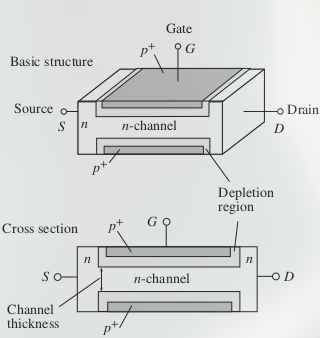
\includegraphics[width=.3\textwidth]{Figures/JFET1}
      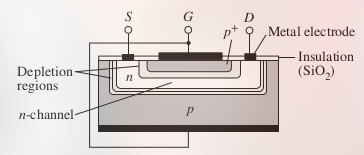
\includegraphics[width=.3\textwidth]{Figures/JFET2}
      \caption{Structure of a $n$-channel JFET, as Depicted in \cite[Page 615]{textbook}}
      \label{fig:1}
    \end{figure}

  \item Metal-Oxide-Semiconductor FET (MOSFET) — A FET constructed with an insulating oxide-based material separating the gate and channel, which results in charges residing on the surface of the conductive material, leading to surface passivization \cite{wiki}, which allows the material to experience less external effects. A sample MOSFET is shown in Figure \ref{fig:2}.

    \begin{figure}[h]
      \centering
      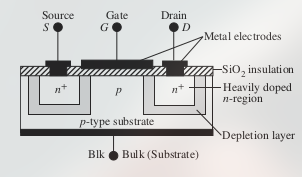
\includegraphics[width=.35\textwidth]{Figures/MOSFET}
      \caption{Structure of an Enhancement MOSFET, as Depicted in \cite[Page 627]{textbook}}
      \label{fig:2}
    \end{figure}

\end{enumerate}

\subsection{Applications of FETs}

The use of FETs has allowed for the development of highly effective integrated circuits, whose functions include, but are not limited to: amplifiers, switches, efficient power electronics, and analog signal processing devices.

\subsection{Key Substrate Material Properties}\label{props}

Given the structure and operating goals of FETs as described above, some key characteristics for applicable high-frequency substrate materials are \cite{young}:

\begin{enumerate}

  \item High Electron Mobility — Higher electron mobility indicates that a material is able to switch more quickly (more efficient operation), as well as operate within a higher frequency range (highly important in modern radio frequency, or RF, applications, and a critical focus of this document).

  \item Lower Effective Mass of Charge Carriers — The need for less charge carrier density for equivalent performance leads to a higher electron mobility, and, as stated in (1), a higher frequency range of operation.

  \item Large Bandgap Width — A larger width in the bandgap results in increased thermal stability and lesser leakage current, which is highly relevant for high frequency devices.

  \item High Thermal Conductivity — The ability to maintain temperature results in greater stability at high frequencies.

\end{enumerate}

As such, we will use these criteria to analyze Gallium Arsenide and Silicon as potential FET substrate materials.

\section{Gallium Arsenide (GaAs)}

\subsection{Fundamental Properties}

Gallium Arsenide, or GaAs, is a material which exhibits a face-centered cubic (or zinc blend) unit crystal structure \cite[Page 104]{textbook}. The unit cell structure is shown in Figure \ref{fig:3}. This structure makes it a highly stable, physically robust material. Furthermore, this kind of structure allows for GaAs to be blended easily with other materials to create alloys, and subsequently heterostructures \cite[Page 568]{textbook}.

\begin{figure}[h]
  \centering
  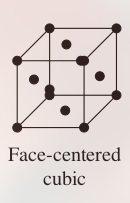
\includegraphics[width=.2\textwidth]{Figures/FCC}
  \caption{Face-Centered Cubic Structure of GaAs \cite[Page 104]{textbook}}
  \label{fig:3}
\end{figure}

GaAs is a highly effective as a semiconductor due to its intrinsic conductivity of $10^{-6}[\si{\ohm\per\meter}]$ \cite[Page 167]{textbook} at room temperature. Despite these advantageous properties, GaAs is subject to several defects due to its crystal structure. For example, a critical point defect which may occur in GaAs is a vacancy (diffusion of an atom to the material surface, leaving a gap to which other atoms diffuse, weakening the structure and conductivity of the overall material) \cite[Page 71]{textbook}. Furthermore, GaAs is subject to dislocations, a line defect which places strain unevenly across the material \cite[Page 75]{textbook}. Though the aforementioned defects are most common, GaAs is also subject to stacking faults (uneven stacking of material planes) and twin boundaries (grain boundaries where crystal orientation shifts), which may result in reduced bandgap width and decreased electron mobility, respectively \cite{GaAsDOE}.

\subsection{Band Structure and Carrier Properties}

GaAs has a direct bandgap of approximately $1.42[\si{eV}]$ at room temperature, which makes it a highly resistive actor when used as a substrate \cite[Page 470]{textbook}, but also very beneficial for its implementation as a light-sensing device or light-emitting diode (LED) \cite[Page 449]{textbook}. The effective electron mass of GaAs is approximately $m^*\approx.067m_e$ \cite[Page 424]{textbook}. Since the electron mobility is inversely proportional to the effective mass of the material per the formula shown in Equation \ref{eq:1}, we may conclude that the low effective mass contributes to GaAs's outstanding electron mobility.

\begin{equation}
  \mu=\frac{q\tau}{m^*}
  \label{eq:1}
\end{equation}

The saturation velocity is the maximum drift velocity attainable by charge carriers (electrons/holes) within the semiconducting material at a maximal electric field strength. Although several factors contribute to the saturation velocity, of most import to us is that higher carrier density yields increased scattering events, which results in a lower saturation velocity (picture more particles per unit volume moving around — this makes collisions more likely, and decreases the average velocity given a maximum electric field). For intrinsic GaAs, we may find the carrier density to be approximately $10^6[\si{\per\centi\meter\cubed}]$, which is fairly low, and, therefore, the saturation velocity is very high. 

\subsection{High-Field Performance}

Of course, when it comes to performance in high-field environments, nothing is more important than a robust breakdown field strength. For GaAs, the breakdown field is approximately $4\cdot10^{5}[\si{\volt\per\centi\meter}]$. Furthermore, with an outstandingly high electron mobility of approximately $8500[\si{\centi\meter\squared\per\volt\per\second}]$ and a large saturation velocity of approximately $1\cdot10^7[\si{\centi\meter\per\second}]$, we may observe that GaAs can operate extremely well in high fields. Due to its robust nature, GaAs is often used to construct high-electron-mobility transistors (HEMT), which are essentially the goal laid out in this document (high frequency FETs).

\subsection{Thermal Considerations}

The thermal conductivity of GaAs is approximately $55[\si{\watt\per\meter\per\kelvin}]$. Though this is good, it is not outstanding relative to other material options. This is, however, stable enough for general use, though high temperature applications may not be as suitable \cite{GaAsDOE}.

\section{Silicon}

\subsection{Fundamental Properties}

Unlike GaAs, which is held together by polar covalent bonds, silicon consists totally of covalent bonding. This total covalent bonding results in a diamond cubic crystal structure, which is essentially the same as the face-centered cubic structure of GaAs, but made with only one material (in this case, silicon. The structure is shown in Figure \ref{fig:4}.

  \begin{figure}[h]
    \centering
    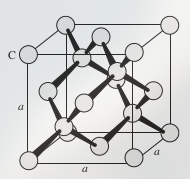
\includegraphics[width=.2\textwidth]{Figures/DCC}
    \caption{Diamond Cubic Crystal Structure \cite[Page 58]{textbook}}
    \label{fig:4}
  \end{figure}

  This material structure leads to many characteristic similarities as GaAs. For example, the defects (and their consequent effects) remain pretty much the same for Silicon: vacancies, dislocations, stacking faults, and twin boundaries can all potentially occur, as well as possible material impurities; however, it is important to note that silicon is subject to oxide contamination, where the surface absorbs moisture, leading to the formation of silicon oxides on the surface of the material \cite{SDef}. The effects of these defects remain the same as in GaAs, namely reduced carrier mobility and increased leakage current.

\subsection{Band Structure and Carrier Properties}

Most importantly, silicon has an indirect bandgap of $1.12[\si{eV}]$ with an effective mass of $m_e^*\approx .26m_e$ \cite[Page 424]{textbook}. Tue, analyzing this in a similar manner as GaAs (using Equation \ref{eq:1}, we see that the electron mobility is thus a quarter of that of GaAs. Similarly, with a carrier density of about $1\cdot10^{10}[\si{\per\centi\meter\cubed}]$, we see that the intrinsic properties of silicon result in lesser carrier mobility (about $1400[\si{\centi\meter\squared\per\volt\per\second}]$ for electrons and $450[\si{\centi\meter\squared\per\volt\per\second}]$ for holes). Due to the greater density of carriers, as we concluded with GaAs, the saturation velocity must be relatively lower, given more particles per volume.

\subsection{High-Field Performance}

Most importantly, we may note that, unlike GaAs, Silicon is highly susceptible to avalanche breakdown \cite[Page 562]{textbook}. Though the exhibit breakdown voltage is similar (within the range of $3$ to $5[\si{\mega\volt\per\centi\meter}]$) this susceptibility makes Silicon less reliable than is gallium-based counterpart. These deficiencies are, in most part, due to the relatively smaller bandgap of Silicon

\subsection{Thermal Considerations}

One field where Silicon shines, however, is its thermal stability. Though the general structure of the Silicon lattice is akin to GaAs, the fact that it consists of a single atom improves its thermal conductivity substantially. Numerically, the thermal conductivity of silicon at room temperature is approximately $150[\si{\watt\per\meter\per\kelvin}]$ \cite{STherm}, or just under three times that of GaAs. Whereas GaAs lacks in applicability for high power electronics due to its lower thermal conductivity, Silicon is able to withstand the heat.

\section{Conclusion}

\subsection{Recommendation}

Overall, we have observed that Silicon and Gallium Arsenide are both highly outstanding materials for use in semiconducting devices. Despite this, Gallium Arsenide's characteristics seem to outshine those of Silicon's, \underline{specifically for use in high frequency FETs}. Constructing a table for easier case-by-case analysis, we may see:

\begin{center}
  \begin{tabular}[H]{|c|c|c|}
    \hline
    & GaAs & Silicon\\
    \hline
    Carrier Mobility $[\si{\centi\meter\squared\per\volt\per\second}]$ & 8500 & 1400\\
    \hline
    Thermal Conductivity $[\si{\watt\per\meter\per\kelvin}]$ & 55 & 150\\
    \hline
    Frequency Response & Faster & Slower\\
    \hline
    Bandgap $[\si{eV}]$ & 1.42 & 1.12\\
    \hline
    Effective Mass $[m_e]$ & .067 & .26\\
    \hline
  \end{tabular}
\end{center}

Let us refer back to Subsection \ref{props}, where the key properties for a high-frequency channel substrate were described. We may observe from the above values that the only property for which Silicon has improved attributes is its thermal conductivity by approximately a factor of 3. Despite this, thermal conductivity is one of the lesser important parameters for high frequency applications, with respect to the others listed. Given Gallium Arsenide's significantly improved carrier mobility, its wider bandgap, and its smaller effective electron mass, when making the choice between either material, it is evident that \underline{Gallium Arsenide is a better candidate for high frequency} \underline{applications}.

\subsection{Trade-Offs}

Despite these findings, it is important to note the use of a more effective material for the aforementioned application does not come without a trade-off. One of the biggest reasons that Silicon continues to be used is that it is a tried and true semiconducting material, popularized around the 1960s, while Gallium Arsenide is a fairly recent development, coming to light in roughly the late 1980s. Furthermore, Gallium Arsenide production remains difficult to scale, causing a significantly higher unit price than Silicon \cite{cost}. Still, newer technologies continue to implement Gallium Arsenide, and, given that production will only get more efficient, it is a surefire outcome that Gallium Arsenide will be used more and more in high frequency applications.

\section*{References}

\begin{thebibliography}{00}
  \bibitem{textbook} S. O. Kasap, Principles of Electronic Materials and Devices, Second Edition. 2001.
  \bibitem{wiki} Wikipedia Contributors, ``Field-effect transistor,'' \textit{Wikipedia}, Oct. 12, 2019. \href{https://en.wikipedia.org/wiki/Field-effect\_transistor}{https://en.wikipedia.org/wiki/Field-effect\_transistor}
  \bibitem{young} M. L. Young and K. C. W. Yu, ``Two-dimensional materials for high-frequency FETs,'' \textit{IEEE Journal of Quantum Electronics}, vol. 55, no. 1, pp. 15-25, Jan. 2020.
  \bibitem{GaAsDOE} U.S. Department of Energy. (2013). ``Material Properties of GaAs'' 
  \bibitem{SDef} V. Gorodokin and D. Zemlyanov, ``Metallic contamination in silicon processing,'' \textit{2004 23rd IEEE Convention of Electrical and Electronics Engineers} in Israel, Tel-Aviv, Israel, 2004, pp. 157-160, doi: 10.1109/EEEI.2004.1361113.
  \bibitem{STherm} H. R. Shanks, P. D. Maycock, P. H. Sidles, and G. C. Danielson, ``Thermal Conductivity of Silicon from 300 to 1400K,'' \textit{Physical Review}, vol. 130, no. 5, pp. 1743–1748, Jun. 1963, doi: https://doi.org/10.1103/physrev.130.1743.
  \bibitem{cost} G. Hiremath and S. Kumar, ``A Comparative Study on Different Semiconductor Materials used for Power Devices and Its Applications'' \textit{International Journal of Latest Technology in Engineering}, vol. VII, 2018, Available: \href{https://www.ijltemas.in/DigitalLibrary/Vol.7Issue1/04-07.pdf}{https://www.ijltemas.in/DigitalLibrary/Vol.7Issue1/04-07.pdf}

‌
\end{thebibliography}

\end{document}
